\documentclass[12pt,a4paper]{article}
\usepackage{ctex}
\usepackage{amsmath,amscd,amsbsy,amssymb,latexsym,url,bm,amsthm}
\usepackage{epsfig,graphicx,subfigure}
\usepackage{enumitem,balance}
\usepackage{wrapfig}
\usepackage{mathrsfs, euscript}
\usepackage[usenames]{xcolor}
\usepackage{hyperref}
\usepackage[vlined,ruled,commentsnumbered,linesnumbered]{algorithm2e}
\usepackage{float}
\usepackage{array}
\usepackage{diagbox}
\usepackage{color}
\usepackage{indentfirst}
\usepackage{fancyhdr}
\usepackage{gensymb}
\usepackage{geometry}
\usepackage{setspace}
\usepackage{aurical}
\usepackage{times}
\usepackage{caption}
\usepackage{fontspec}
\usepackage{booktabs}
\usepackage{listings}
\usepackage{xcolor}
\setmainfont{Times New Roman}

\newtheorem{theorem}{Theorem}[section]
\newtheorem{lemma}[theorem]{Lemma}
\newtheorem{proposition}[theorem]{Proposition}
\newtheorem{corollary}[theorem]{Corollary}
\newtheorem{exercise}{Exercise}[section]
\newtheorem*{solution}{Solution}
\theoremstyle{definition}

\newcommand{\tabincell}[2]{\begin{tabular}{@{}#1@{}}#2\end{tabular}}
\newcommand{\postscript}[2]
 {\setlength{\epsfxsize}{#2\hsize}
  \centerline{\epsfbox{#1}}}

\renewcommand{\baselinestretch}{1.05}

\setlength{\oddsidemargin}{-0.365in}
\setlength{\evensidemargin}{-0.365in}
\setlength{\topmargin}{-0.3in}
\setlength{\headheight}{0in}
\setlength{\headsep}{0in}
\setlength{\textheight}{10.1in}
\setlength{\textwidth}{7in}
\makeatletter \renewenvironment{proof}[1][Proof] {\par\pushQED{\qed}\normalfont\topsep6\p@\@plus6\p@\relax\trivlist\item[\hskip\labelsep\bfseries#1\@addpunct{.}]\ignorespaces}{\popQED\endtrivlist\@endpefalse} \makeatother
\makeatletter
\renewenvironment{solution}[1][Solution] {\par\pushQED{\qed}\normalfont\topsep6\p@\@plus6\p@\relax\trivlist\item[\hskip\labelsep\bfseries#1\@addpunct{.}]\ignorespaces}{\popQED\endtrivlist\@endpefalse} \makeatother

\begin{document}
\noindent
%==========================================================
\noindent\framebox[\linewidth]{\shortstack[c]{
\Large{\emph{模型评价与模型改善}}\vspace{1mm}\\
CS245 \quad 数据科学基础 \quad 陆朝俊}}

\section{问题描述}

给定一个机器学习问题(如分类)以及相应的数据集,可以训练出一个初步的模型,但在投入实际应用前,需要对该模型的性能进行评价甚至改善。一般地,通过组合模型的方式,可以提高模型的效果。这次作业中,我将在自己建立的数据集上探索决策树模型单独工作以及组合工作时的分类性能。

\section{解决方案\protect\footnote{本次作业的主要代码实现可参见附录 \ref{apd:code}}}

\subsection{数据集的建立及模型的选择}

由于现有的中小型数据集存在一些难以满足实验要求的属性,我选择自己建立一个分类数据集$D$(后文均以$D$表示此数据集),之后的所有实验均基于此数据集上进行。数据集$D$包含500个样本,30个特征(存在冗余和重复的特征),为更好地看出模型性能的区别,我在$D$中添加了部分噪声。关于数据集$D$详细的设定参数可参考附录 \ref{apd:dataset_para}。

\vspace{0.015\linewidth}
解决分类问题的机器学习模型主要有逻辑回归、决策树以及KNN等,在这次作业中,我选择决策树作为探索的模型。

\subsection{探索模型单独工作的性能}

选定数据集和模型后,我首先探索单独的决策树模型在数据集$D$上的分类性能,探索方法如下:

\begin{enumerate}
\item \textbf{直接划分训练集和测试集}

在一般应用中,对模型性能最朴素的评价方法即为:将数据集划分为训练集和测试集,在训练集上训练模型后,根据模型在测试集上的表现评价模型性能。因此,我首先采用这个方法对模型的性能进行一个粗略的估计。

\item \textbf{分层交叉验证}

从理论上说,仅凭在一个训练集$D_1$上训练出的模型$M_1$无法代表模型$M$(在我的实验中为决策树模型)解决这个问题的效果。分层交叉验证正好解决了这一问题,其步骤大致如下:

\begin{enumerate}
	\item 将数据随机等分为$k$个不相交子集$D_1, D_2, ... ,D_k$(每个子集的类分布与初始数据近似相同);
	
	\item 总共执行$k$次训练与测试,在第$i$折时,使用$D_i$作为测试集, 其他子集作为训练集;
	
	\item 模型的性能由$k$次迭代的平均效果决定。
\end{enumerate}

分层交叉验证相当于在同一个数据集上进行了多次训练集-测试集划分。和简单的训练集-测试集划分相比,能更准确地评估模型来自样本的误差。

\item \textbf{网格搜索}

网格搜索是指通过蛮力试验不同参数组合,从而选择最佳模型的方法。理论上来说,网格搜索与分层交叉验证相结合,可以找出模型解决给定问题最合适的参数,但这一过程需要花费大量的时间和计算资源,因此这次作业中我仅实现了一小部分参数空间上的网格搜索。

\end{enumerate}

\subsection{探索模型组合工作的性能}

一般地,从一系列模型$M_1, M_2, ... , M_k$创建组合模型$M^*$,可以有效提高原模型的效果。组合方法主要有bagging、boosting、voting和stacking等,本次作业我探索了bagging和boosting两种组合方法的效果。

\vspace{0.01\linewidth}
Bagging方法使用并行思想,$M^*$通过整合各原模型的结果得到输出;Boosting方法则采用串行思想,不断利用模型$M_{i-1}$的训练结果训练模型$M_{i}$,以最小化目标函数(损失函数),直到$M_k$,属于一种迭代搜索算法。

\section{实验及结果}

\subsection{模型单独工作的性能}
\label{sec:pca_res_com}

\subsubsection{直接划分训练集和测试集}

首先,我将原数据按照一定比例划分为训练集和测试集,划分时保证\textbf{每一类型的数据在训练集和测试集的占比大致服从原分布},再执行一般的“训练集上训练-测试集上测试”流程。测试结果如表 \ref{tab:train-test} 所示。

\begin{table}[H]
	\renewcommand\arraystretch{1.35}
	\caption{不同比例的训练集-测试集划分下,决策树模型在$D$上的性能}
	\label{tab:train-test}
	\centering
	
	\begin{tabular}{c|c|c|c|c}
		\centering
		\tabincell{c}{测试集占比(其中\\0表示随机分类)} & \tabincell{c}{测试集上平均\\精确度} & \tabincell{c}{测试集上平均\\召回率} & \tabincell{c}{测试集上平均\\f1-score} & \tabincell{c}{训练集上平均\\f1-score} \\
		\hline
		0 & 0.38 & 0.36 & 0.36 & 0.33 \\
		0.05 & 0.78 & 0.72 & 0.73 & 1.00 \\
		0.1 & 0.59 & 0.56 & 0.56 & 1.00 \\
		0.2 & 0.57 & 0.56 & 0.56 & 1.00 \\	
		0.3 & 0.57 & 0.56 & 0.56 & 1.00 \\	
		0.4 & 0.56 & 0.56 & 0.55 & 1.00 \\
		0.5 & 0.50 & 0.48 & 0.48 & 1.00 \\
		0.8 & 0.49 & 0.48 & 0.48 & 1.00 \\
	\end{tabular}
\end{table}

粗略测试的结果表明:不论训练集-测试集的划分比例如何,该模型总是表现为低偏差、高方差,趋于过拟合,对新数据的分类效果较差。

\subsubsection{分层交叉验证}

上小节仅对决策树模型在$D$上单独工作的性能进行了粗略的估计,下面使用分层交叉验证对模型单独工作的性能做更完整的探索,结果参见图 \ref{fig:cv_bar}。

\begin{figure}[H]
	\centering
	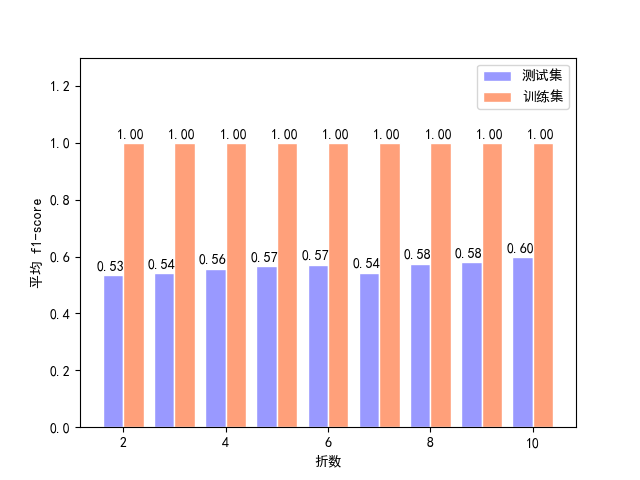
\includegraphics[width=0.8\linewidth]{img/cv_bar.png}
	\caption{分层交叉验证探索模型在$D$上的性能}
	\label{fig:cv_bar}
\end{figure}

从图中可以看出,折数和在测试集上的f1-score呈正相关(折数越多,训练集则越大,模型对$D$学习得更充分),但均在0.5与0.6之间,对于一般应用来说也属于较低水平。除此之外,图中低偏差和高方差的表现也说明模型的过拟合问题尤为严重。

\subsubsection{网格搜索}

这部分实验中,我结合网格搜索和分层交叉验证(10折),得到决策树模型在$D$上的最佳效果。由于遍历所有参数需要消耗大量的时间和计算资源,我在实验中仅选择了模型的部分重要参数进行网格搜索。具体结果可参见表 \ref{tab:grid-search}。

\begin{table}[H]
	\renewcommand\arraystretch{1.35}
	\caption{网格搜索结果}
	\label{tab:grid-search}
	\centering
	
	\begin{tabular}{c|c|c|c}
		\centering
		参数名 & 参数含义 & 参数范围 & 模型效果最佳时的值 \\
		\hline
		criterion & 特征选择的度量标准 & gini, entropy & gini \\
		\hline
		max\_depth & 树的最大深度 & 正整数 & 9 \\
		\hline
		max\_features & \tabincell{c}{寻求最佳划分时\\要考虑的特征数目} & \tabincell{c}{总特征数或其平方根\\或其以2为底的对数值} & 总特征数 \\
		\hline
		presort & 是否对数据预先排序 & True, False & True \\
		\hline
		splitter & 结点划分策略 & best, random & best \\
	\end{tabular}
\end{table}

经过对上表参数值的网格搜索,得到的模型在分层交叉验证中各测试集的平均f1-score为0.61,虽然只遍历了一部分参数空间,但这个结果在一定程度上也能够代表决策树模型在$D$上分类的最佳性能。最佳模型的可视化结果可参见附录 \ref{apd:vis-tree}。

\subsubsection{结果分析}

通过上面三个小节的探索,可以得出结论:决策树模型单独工作时,在数据集$D$上分类的f1-score基本在0.5-0.6之间,最高仅达0.61,而在训练集上的分类效果极佳,表明该模型在$D$上单独工作时容易趋于过拟合,对新数据的分类效果较差,即低偏差、高方差。

\subsection{模型组合工作的性能}
\label{sec:bagging}

在这一节的实验中,我主要探索了决策树模型在bagging和boosting两种组合方式下于数据集$D$上的分类性能,以f1-score为分类的评价标准。

\subsubsection{Bagging}

Bagging方法整合各子模型的输出从而得到结果,因此每个子模型的训练方式对最终结果也有较大的影响。一般地,在训练子模型时选择合适的特征比例(即舍去训练数据的部分特征)可以降低过拟合程度,得到良好的模型。这部分实验中,我选择了\textbf{不同子模型个数}以及\textbf{不同比例的特征}进行训练,之后采用10折分层交叉验证对bagging整合后的模型进行性能评价,结果可参见图 \ref{fig:bagging}。

\vspace{-0.015\linewidth}
\begin{figure}[H]
	\centering
	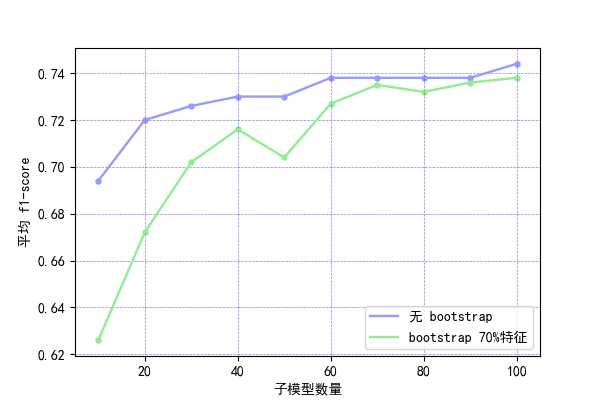
\includegraphics[width=0.8\linewidth]{img/bagging_kline.png}
	\caption{Bagging组合模型在测试集上的性能(在训练集上的f1-score均为1,因此不再画出)}
	\label{fig:bagging}
\end{figure}

从上图中易知:Bagging组合模型性能与子模型个数大致呈正相关。同时对比图 \ref{fig:cv_bar} 和图 \ref{fig:bagging} 的结果,可以发现经过bagging组合的模型在测试集上能够达到更高的f1-score(最高0.74左右),减小了模型的方差。但经bagging组合后的模型仍在一定程度上存在过拟合的问题,相关讨论可见 \ref{sec:dis} 小节。

\vspace{0.015\linewidth}
为探索每个子模型对特征的提取结果,我将其可视化于图 \ref{fig:bagging-feature}。图中各点的分布表明:虽然有些子模型抽取的特征相似,但大部分抽取的特征分布相差较大,因此整合各模型的预测结果是有意义的。

\begin{figure}[H]
	\centering
	\subfigure[5个子模型]{
		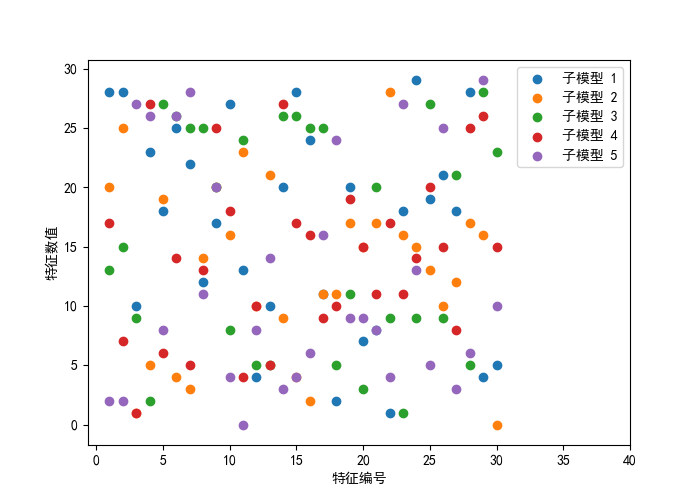
\includegraphics[width=0.31\linewidth]{img/bagging_feature_5.png}
	}
	\subfigure[10个子模型]{
		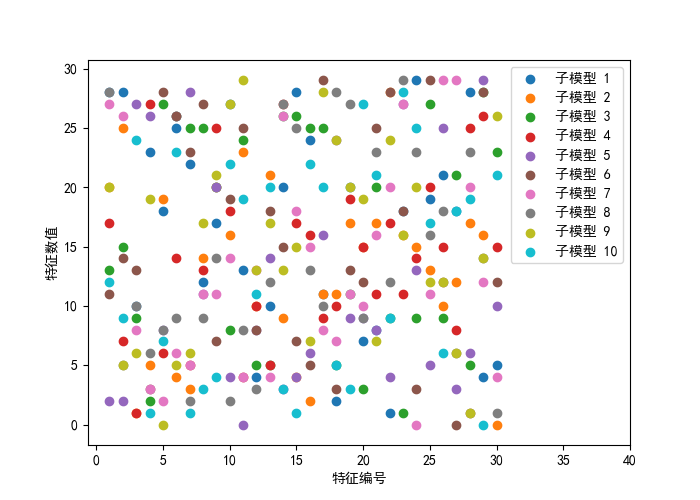
\includegraphics[width=0.31\linewidth]{img/bagging_feature_10.png}
	}
	\subfigure[15个子模型]{
		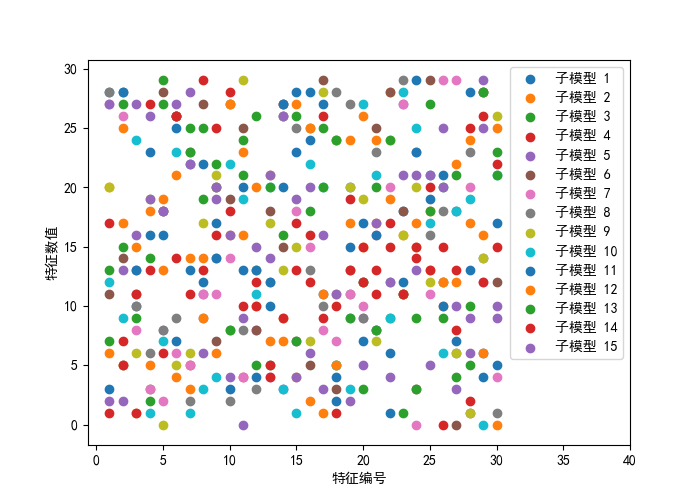
\includegraphics[width=0.31\linewidth]{img/bagging_feature_15.png}
	}
	\caption{Bagging子模型特征可视化}
	\label{fig:bagging-feature}
\end{figure}

\vspace{-0.05\linewidth}
\subsubsection{Boosting}
\label{sec:boosting}

Boosting不断地使用子模型弥补前一个子模型的“不足”,串行地构造一个强模型。具体的实现主要有Adaboost、SAMME和SAMME.R等。这部分实验中,我使用SAMME和SAMME.R算法探索了在不同子模型个数下,boosting组合模型在10折分层交叉验证下的性能,结果参见图 \ref{fig:boosting}。

\vspace{-0.03\linewidth}
\begin{figure}[H]
	\centering
	\subfigure[训练集]{
		\label{fig:boosting-train}
		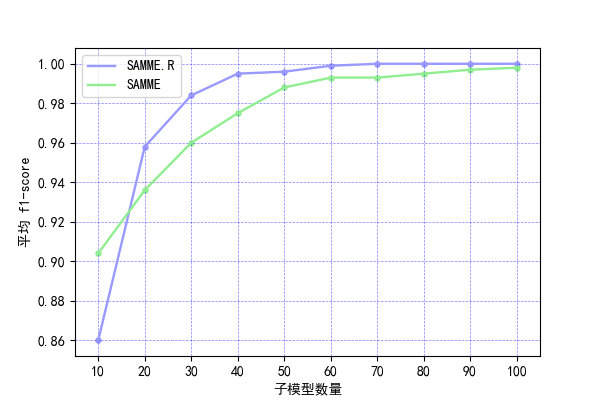
\includegraphics[width=0.48\linewidth]{img/boosting_kline_train.png}
	}
	\subfigure[测试集]{
		\label{fig:boosting-test}
		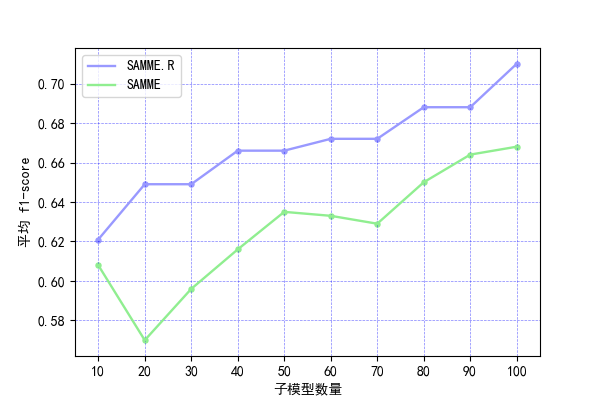
\includegraphics[width=0.48\linewidth]{img/boosting_kline_test.png}
	}
	\caption{Boosting组合模型性能}
	\label{fig:boosting}
\end{figure}

\vspace{-0.012\linewidth}
从上图可以看出:1)组合模型的性能与子模型个数大致呈正相关;2)和模型单独工作相比,boosting方法同样提升了模型的性能,尤其是降低了模型的方差。对比图 \ref{fig:bagging} 及图 \ref{fig:boosting-test} 的结果可知,bagging和boosting在测试集上平均f1-score的变化趋势和最终数值基本一致。但结合boosting在训练集上的效果(图 \ref{fig:boosting-train} )分析,boosting相对于单独模型和bagging方法,过拟合程度更低,保证模型低偏差的同时减小了模型的方差。

\vspace{0.012\linewidth}
各子模型的权重与错误率的关系见图 \ref{fig:boosting-weight-error}。

\vspace{-0.012\linewidth}
\begin{figure}[H]
	\centering
	\subfigure[5个子模型]{
		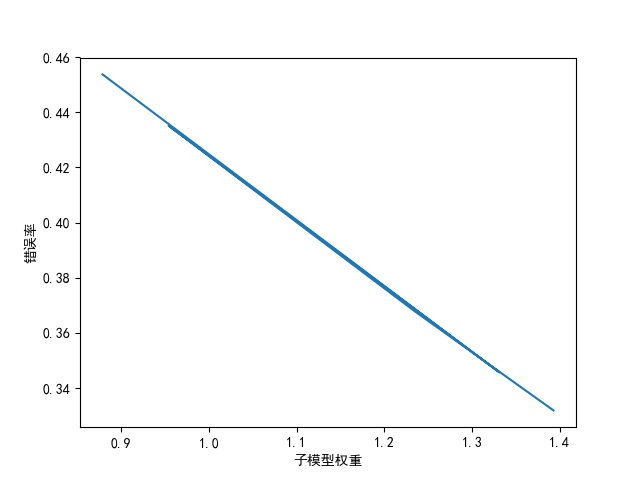
\includegraphics[width=0.31\linewidth]{img/boosting-weight-error-5.png}
	}
	\subfigure[10个子模型]{
		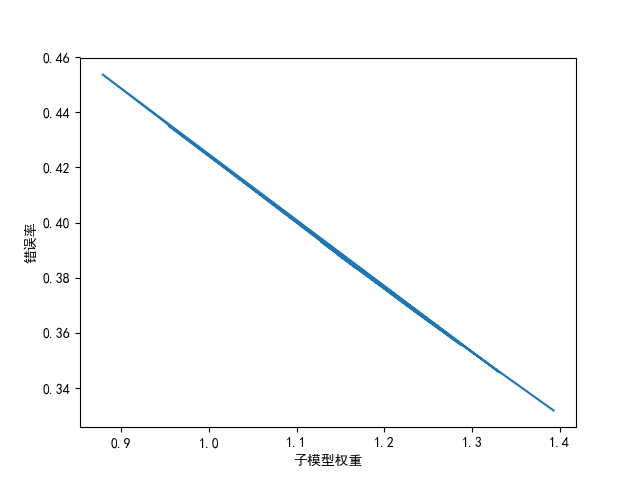
\includegraphics[width=0.31\linewidth]{img/boosting-weight-error-10.png}
	}
	\subfigure[15个子模型]{
		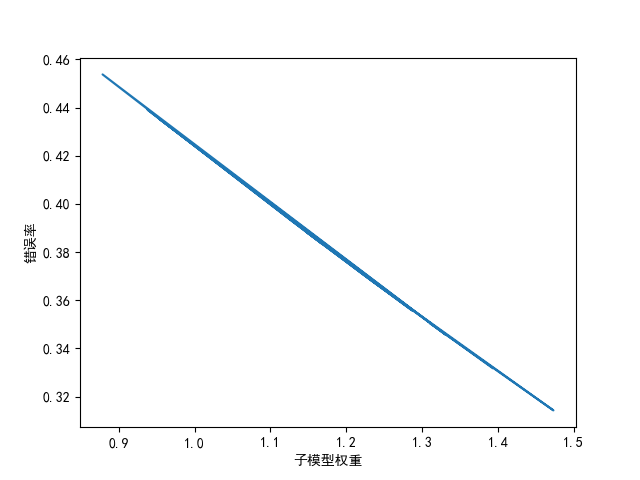
\includegraphics[width=0.31\linewidth]{img/boosting-weight-error-15.png}
	}
	\caption{Boosting子模型的权重与错误率关系}
	\label{fig:boosting-weight-error}
\end{figure}

\subsubsection{结果分析}
\label{sec:dis}

Bagging和boosting虽然都属于组合模型的方法,都能够改进模型的性能,但其背后不同的思想决定了它们对模型的改进有着不同的侧重点。

\vspace{0.015\linewidth}
Bagging充分利用了不同子模型的预测结果,有利于模型的互补,通过\textbf{降低模型方差}改善性能;Boosting则通过多步迭代,不断优化目标函数,将弱模型逐步转化成强模型,因此和bagging相比,boosting一般能得到\textbf{更高的准确度}(即更低的偏差),但也存在模型过拟合的风险(即更高的方差)。

\vspace{0.015\linewidth}
然而, \ref{sec:bagging} 和 \ref{sec:boosting} 小节的结果与上面的理论分析似乎存在矛盾:Bagging方法在降低方差上并没有显著的表现,而boosting方法的偏差和bagging相比,也不存在明显的优势,反而能够在一定程度上降低过拟合程度。

\vspace{0.015\linewidth}
经过分析,我认为这一结果的背后存在多个原因:

\begin{enumerate}

\item \textbf{参数设置  } Bagging和boosting属于不同思想的算法,参数的种类也不同,难以在相同条件下对二者进行比较。二者参数中包含大量连续型参数(如bagging中的特征取样比例、boosting中的学习率),这也使得网格搜索无法实现。因此,对于两种组合算法性能的比较,无法统一在相同的条件下,只能从理论上分析出大致的结果,对具体的问题而言可能各有不同。

\item \textbf{子模型的类型  } 实验中选择的分类模型是决策树模型,bagging方法虽然利用不同的训练样本引入随机成分,训练了多个决策树模型,但这些树之间仍存在相关性,尤其是树的上层,几乎具有相同的结构,将这些结构相似的模型进行组合,对方差的降低自然无法体现。而低偏差、高方差,易过拟合也是决策树本身所具有的特点。采用随机森林(分割结点时将特征也做随机选取)算法,可以有效解决这一问题。

\item \textbf{数据的影响  } 在这次实验中,为了使模型性能的提升更加明显,我在数据集中添加了冗余特征、重复特征甚至噪音(见附录 \ref{apd:dataset_para}),加大了分类难度。这些数据上的干扰也在一定程度限制了各种方法的性能,导致实验结果与理论有些许偏差。

\end{enumerate}

\section{结论}

综上,决策树模型在数据集$D$上单独工作时,偏差较低而方差较大,即在训练集上表现极佳,但在新数据上效果较差。和单独工作相比,模型组合工作时,无论是bagging还是boosting方法都能够在保证低偏差的情况下有效降低模型的方差,其中boosting组合模型的偏差比bagging稍高,而方差稍低。但由于决策树模型本身的特点影响,加上数据集存在噪音以及参数未经过大量调整,即使是组合模型也难以满足实际应用的性能需求。

\newpage
\begin{appendix}
	\section{附录}
	\subsection{分类数据集$D$的详细信息}
	\label{apd:dataset_para}
	\begin{table}[H]
		\renewcommand\arraystretch{1.35}
		\caption{分类数据集$D$的详细信息}
		\label{tab:dataset_para}
		\centering
		
		\begin{tabular}{c|c}
			\centering
			属性 & 值 \\
			\hline
			样本个数 & 50 \\
			特征个数 & 30 \\
			类个数 & 3 \\
			类分布 & 每个类均匀分布 \\
			包含信息的特征占比 & 0.6 \\
			冗余特征的占比(含信息特征的线性组合) & 0.1 \\
			重复特征的占比(随机取自含信息特征和冗余特征) & 0.1 \\
			噪声占比 & 0.03 \\		
		\end{tabular}
	\end{table}
	
	\subsection{决策树单独工作的最佳模型可视化}
	由于图片较大,若有需要可放大后详细观看,不影响图片清晰度。
	\label{apd:vis-tree}
	\begin{figure}[H]
		\centering
		
\includegraphics[width=0.9\linewidth]{img/gs.pdf}
		\caption{决策树单独工作的最佳模型}
	\end{figure}
	
	\subsection{主要代码}
	\label{apd:code}
	
	\begin{lstlisting}[language=Python,
	numbers=left,
	keywordstyle=\color{blue!70},
	frame=shadowbox,
	breaklines=True]
from sklearn.cross_validation import StratifiedKFold
from sklearn.datasets import make_classification
from sklearn.cross_validation import train_test_split
from sklearn.metrics import classification_report

from sklearn.tree import export_graphviz
from sklearn.tree import DecisionTreeClassifier
from sklearn.ensemble import BaggingClassifier
from sklearn.ensemble import AdaBoostClassifier
from sklearn.grid_search import GridSearchCV

import numpy as np
import matplotlib.pyplot as plt
plt.rcParams['font.sans-serif']=['SimHei']
plt.rcParams['axes.unicode_minus']=False

##################### making dataset ######################

n = 500                 # number of instances
n_f = 30                # number of features
n_c = 3                 # number of classes
inf_f = int(0.6 * n_f)  # 60% real features
red_f = int(0.1 * n_f)  # 10% redundant features
rep_f = int(0.1 * n_f)  # 10% repeated features
random_seed = 1         # random seed for the experiments

X, Y = make_classification(n_samples=n, n_classes=n_c, flip_y=0.03,
                    n_features=n_f, n_informative=inf_f, n_redundant=red_f,
                    n_repeated=rep_f, random_state=random_seed)
X_train, X_test, Y_train, Y_test = \
    train_test_split(X, Y, test_size=0.8, random_state=random_seed)

##################### making dataset ######################

# directly train the model with training set & testing set
def exp_plain_train():
    model = DecisionTreeClassifier(random_state=random_seed)
    model.fit(X_train, Y_train)

    pred = model.predict(X_test)
    print(classification_report(Y_test, pred))

    score = model.score(X_test, Y_test)
    print('plain train score in testing set: ', score)
    score = model.score(X_train, Y_train)
    print('plain train score in training set: ', score)

# test model with cross-validation
def exp_cv(folds=10):
    kfolds = StratifiedKFold(Y, n_folds=folds, random_state=random_seed)
    model = DecisionTreeClassifier(random_state=random_seed)
    scores_train = []
    scores_test = []
    for train, test in kfolds:
        model.fit(X[train], Y[train])
        # pred = model.predict(X[test])

        score = model.score(X[test], Y[test])
        scores_test.append(score)
        score = model.score(X[train], Y[train])
        scores_train.append(score)

    mean_test = np.array(scores_test).mean()
    mean_train = np.array(scores_train).mean()
    print('avg score with cv folds %d in testing set: '
          % folds, mean_test)
    print('avg score with cv folds %d in training set: '
          % folds, mean_train)

    return mean_test, mean_train

def plot_cv():
    mean_tests = []
    mean_trains = []
    folds_sum = 11
    for i in range(2, folds_sum):
        m1, m2 = exp_cv(i)
        mean_tests.append(m1)
        mean_trains.append(m2)

    # start to plot
    x = np.arange(2, folds_sum)
    total_width, n = 0.8, 2
    width = total_width / n
    x = x - (total_width - width) / 2

    plt.bar(x, mean_tests, width=width,
            facecolor='#9999ff', edgecolor='white', label=u'测试集')
    plt.bar(x + width, mean_trains, width=width,
            facecolor='#ffa07a', edgecolor='white', label=u'训练集')
    for x, y1, y2 in zip(x, mean_tests, mean_trains):
        plt.text(x - 0.05, y1 + 0.01, '%.2f' % y1, ha='center', va='bottom')
        plt.text(x+width - 0.05, y2 + 0.01, '%.2f' % y2, ha='center', va='bottom')

    plt.xlabel(u'折数')
    plt.ylabel(u'平均 f1-score')
    plt.ylim((0, 1.3))
    plt.legend()
    plt.savefig('report/img/cv_bar')
    plt.show()

# grid search
def exp_grid_search(folds=10):
    model = DecisionTreeClassifier(random_state=random_seed)
    param_grid = {'criterion': ['gini', 'entropy'],
                  'max_features': ['sqrt', 'log2', None],
                  'max_depth': list(range(3, 15)),
                  'presort': [True, False],
                  'splitter': ['best', 'random']
                  }
    grid = GridSearchCV(model, param_grid, cv=folds, scoring='f1_weighted')
    grid.fit(X, Y)

    print(grid.best_params_)
    print(grid.best_score_)

    export_graphviz(grid.best_estimator_, filled=True, out_file='report/img/gs.dot')

# bagging alg
def bagging(cv=True):
    bagging = BaggingClassifier(
        DecisionTreeClassifier(random_state=random_seed),
        n_estimators=5,            # number of models
        random_state=random_seed,
        bootstrap=True,
        max_samples=1.0,            # Bootstrap sample size radio
        bootstrap_features=True,
        max_features=1.0,           # Bootstrap feature usage radio
    )
    if cv:          # using cross-validation
        scores_train = []
        scores_test = []
        kfolds = StratifiedKFold(Y, n_folds=10, random_state=random_seed)
        for train, test in kfolds:
            bagging.fit(X[train], Y[train])

            score = bagging.score(X[test], Y[test])
            scores_test.append(score)
            score = bagging.score(X[train], Y[train])
            scores_train.append(score)

        mean_test = np.array(scores_test).mean()
        mean_train = np.array(scores_train).mean()
        print('avg score with cv folds 10 in testing set: ', mean_test)
        print('avg score with cv folds 10 in training set: ', mean_train)
    else:           # without cross-validation
        bagging.fit(X_train, Y_train)
        pred = bagging.predict(X_test)
        print(classification_report(Y_test, pred))

    # check the features extracted by each model
    plt.figure(figsize=(7, 5))
    f_n = 30
    x = list(range(1, f_n + 1))
    for i, f in enumerate(bagging.estimators_features_):
        print('model %d' % (i + 1), f)
        plt.scatter(x, f, label=u'子模型 %d' % (i + 1))
    plt.xlabel(u'特征编号')
    plt.xticks(list(range(0, 41, 5)))
    plt.ylabel(u'特征数值')
    plt.legend(loc=1)
    plt.savefig('report/img/bagging_feature_%d' % len(bagging.estimators_features_))
    plt.show()

def plot_bagging():
    # results
    x = list(range(10, 101, 10))
    y = [0.694, 0.720, 0.726, 0.730, 0.730, 0.738, 0.738, 0.738, 0.738, 0.744]
    y_b1 = [0.626, 0.672, 0.702, 0.716, 0.704, 0.727, 0.735, 0.732, 0.736, 0.738]
    y_b2 = [0.668, 0.711, 0.738, 0.734, 0.744, 0.746, 0.738, 0.730, 0.740, 0.738]

    # ploting code
    plt.figure(figsize=(6, 4))
    ax = plt.gca()
    ax.plot(x, y_b1, color='#90EE90', linewidth=1.7, label=u'70%特征')
    ax.plot(x, y_b2, color='#ffa07a', linewidth=1.7, label=u'90%特征')
    ax.plot(x, y, color='#9999ff', linewidth=1.7, label=u'100%特征')
    ax.scatter(x, y, s=13, c='#9999ff')
    ax.scatter(x, y_b1, s=13, c='#90EE90')
    ax.scatter(x, y_b2, s=13, c='#ffa07a')
    ax.grid(color='b', alpha=0.5, linestyle='dashed', linewidth=0.5)
    plt.xlim((5, 105))
    plt.xticks(x)
    plt.xlabel(u'子模型数量')
    plt.ylabel(u'平均 f1-score')
    plt.legend()
    plt.savefig('report/img/bagging_kline')
    plt.show()

# boosting alg
def boosting(cv=True):
    boosting = AdaBoostClassifier(
        DecisionTreeClassifier(max_depth=3, min_samples_leaf=2, random_state=random_seed),
        n_estimators=15,   # number of models
        algorithm='SAMME',  # Advanced-Boosting
        random_state=random_seed
    )
    if cv:      # using cross-validation
        scores_train = []
        scores_test = []
        kfolds = StratifiedKFold(Y, n_folds=10, random_state=random_seed)
        for train, test in kfolds:
            boosting.fit(X[train], Y[train])

            score = boosting.score(X[test], Y[test])
            scores_test.append(score)
            score = boosting.score(X[train], Y[train])
            scores_train.append(score)

        mean_test = np.array(scores_test).mean()
        mean_train = np.array(scores_train).mean()
        print('avg score with cv folds 10 in testing set: ', mean_test)
        print('avg score with cv folds 10 in training set: ', mean_train)
    else:       # without cross-validation
        boosting.fit(X_train, Y_train)

        pred = boosting.predict(X_train)
        print(classification_report(Y_train, pred))

        pred = boosting.predict(X_test)
        print(classification_report(Y_test, pred))

    # plot the relation between weights and error
    plt.figure()
    plt.xlabel(u'子模型权重')
    plt.ylabel(u'错误率')
    plt.plot(boosting.estimator_weights_, boosting.estimator_errors_)
    plt.savefig('report/img/boosting-weight-error-%d' % len(boosting.estimator_weights_))
    plt.show()

def plot_boosting():
    # results
    x = list(range(10, 101, 10))
    y1 = [0.621, 0.649, 0.649, 0.666, 0.666, 0.672, 0.672, 0.688, 0.688, 0.710]
    y2 = [0.608, 0.570, 0.596, 0.616, 0.635, 0.633, 0.629, 0.650, 0.664, 0.668]
    y1_tr = [0.860, 0.958, 0.984, 0.995, 0.996, 0.999, 1.000, 1.000, 1.000, 1.000]
    y2_tr = [0.904, 0.936, 0.960, 0.975, 0.988, 0.993, 0.993, 0.995, 0.997, 0.998]

    # plot testing results
    plt.figure(figsize=(6, 4))
    ax = plt.gca()
    ax.plot(x, y1, color='#9999ff', linewidth=1.7, label='SAMME.R')
    ax.plot(x, y2, color='#90EE90', linewidth=1.7, label='SAMME')
    ax.scatter(x, y1, s=13, c='#9999ff')
    ax.scatter(x, y2, s=13, c='#90EE90')
    ax.grid(color='b', alpha=0.5, linestyle='dashed', linewidth=0.5)
    plt.xlim((5, 105))
    plt.xticks(x)
    plt.xlabel(u'子模型数量')
    plt.ylabel(u'平均 f1-score')
    plt.legend()
    plt.savefig('report/img/boosting_kline_test')
    plt.show()

    # plot training results
    plt.figure(figsize=(6, 4))
    ax = plt.gca()
    ax.plot(x, y1_tr, color='#9999ff', linewidth=1.7, label='SAMME.R')
    ax.plot(x, y2_tr, color='#90EE90', linewidth=1.7, label='SAMME')
    ax.scatter(x, y1_tr, s=13, c='#9999ff')
    ax.scatter(x, y2_tr, s=13, c='#90EE90')
    ax.grid(color='b', alpha=0.5, linestyle='dashed', linewidth=0.5)
    plt.xlim((5, 105))
    plt.xticks(x)
    plt.xlabel(u'子模型数量')
    plt.ylabel(u'平均 f1-score')
    plt.legend()
    plt.savefig('report/img/boosting_kline_train')
    plt.show()

if __name__ == '__main__':
    # exp_plain_train()
    # exp_cv()
    # plot_cv()
    # exp_grid_search()
    boosting()
    # plot_boosting()
    # bagging()
    # plot_bagging()
	\end{lstlisting}
	
\end{appendix}

%========================================================================
\end{document}